\shorthandoff{'}
\begin{markdown*}{%
  hybrid,
  definitionLists,
  footnotes,
  inlineFootnotes,
  hashEnumerators,
  fencedCode,
  citations,
  citationNbsps,
  pipeTables,
  tableCaptions,
}

\chapter{Motivation}

Microcontrollers in embedded devices are typically programmed in compiled languages like C, C++, or Rust. Although these languages provide high performance and low overhead at runtime, they can be challenging to learn and use.

Another problem of compiled languages, especially in embedded environments, is a long development cycle. Because of the limited resources of a microcontroller, the executable of such applications is usually self-contained to decrease the binary size and to avoid the need for a dynamic linker. Besides the application itself, such executables contain all used libraries, including the standard ones. All libraries must be linked on every build and, in some cases, also compiled regardless of whether they have changed.

The development cycle is often further prolonged by long deployment times. The build-deploy process can take several minutes, compromising development speed, especially in the early development stages when the developer rapidly iterates over the code.

The long development cycle can both hinder development speed and increase the development cost. Another big motivator for reducing the development cycle length is teaching beginners embedded programming. Seeing the results of their work quickly is important for keeping the learners motivated and interested in the subject, especially with children and their shorter attention spans.

As embedded devices often interact with the outside world or communicate with other devices, they often have to wait for external events rather than continuously perform a given computation. Therefore, most embedded applications have reactive and asynchronous elements, which are difficult to express in low-level languages. This induces a lot of boilerplate code, which obfuscates the main application logic and makes it harder to develop and maintain. Even though high-level languages such as C++ and Rust somewhat alleviate this issue, C is often the only language with direct support from the manufacturers, which adds more work for the developer and more code to the project.


\chapter{Proposed solution}

The proposed solution is to use a high-level, interpreted language instead. The language needs to:

  - have low enough hardware requirements to run on a microcontroller,
  - be easy to learn and use, and
  - be able to express reactive and asynchronous elements.

\noindent
The solution should also provide an ecosystem for controlling the device and developing applications. The ecosystem should include:

  - firmware for the microcontroller, which gives complete control over the device to the runtime environment and provides an interface for controlling the device, and
  - suitable tooling for controlling the device and uploading code to it.

\section{Language choice}

Many interpreted languages are available. Because of their popularity in embedding into other applications, the following languages were considered:

  - Python
  - Lua
  - JavaScript

Python is a general-purpose language with an extensive standard library, which makes it suitable for many applications. However, its high hardware requirements caused by its large standard library and its memory model make it unsuitable for embedded devices.

Lua is a lightweight scripting language with a small standard library. It is suitable for embedded devices, and there are efficient Lua interpreters which are embeddable into C/C++ applications. On the other hand, Lua is not nearly as popular as Python or JavaScript, making it harder to find relevant resources and justify learning a new language.

JavaScript is a popular language commonly used in web browsers. The language specification defines a small standard library, which is extended by the runtime environment, meaning a small base memory footprint. It also maps very well to the event-centered nature of many embedded systems, as JavaScript is inherently event-driven. Multiple embeddable JavaScript engines exist, such as DukTape, MuJS, and QuickJS.

Because of the reasoning above, JavaScript was chosen to be used in the solution implemented in this thesis.

However, since JavaScript is weakly typed, debugging errors caused by type mismatches can be challenging. A possible solution is to use a strongly typed language, such as TypeScript. However, as transpiling\footnote{Transpilation refers to the process of source-to-source compilation} or interpreting TypeScript on a microcontroller is not feasible, it must first be transpiled to JavaScript outside of the device.


\chapter{Overview}

The main task is to create a JavaScript runtime environment for microcontrollers and an ecosystem around it for managing the device and developing applications for it.

The implementation primarily focuses on the ESP32 and ESP32-S3 series microcontrollers, as they are popular in the maker community and provide high performance at a reasonably low price. Because of their extensive feature set, they also serve as a good entry point for beginners, who can try out many different things with a single device.

Firmware for microcontrollers, which gives complete control over the device to the JavaScript runtime and provides an interface for programming and controlling the device, should be developed. A device running this firmware will be called a *Jaculus device*.

\section{Runtime environment}

The runtime environment should be able to run JavaScript code and be easily extensible with functionality implemented in C++. The runtime should be usable as the primary interface for programming the device and as a component of a larger application.

An example use case for the latter is in a system of devices used as game elements. Their low-level logic (e.g., communication, user interface) can be implemented in C++, while the high-level logic (e.g., game rules) can be updated independently by the user.

\section{JavaScript engine}

A JavaScript engine is needed to interpret JavaScript code. As implementing a custom JavaScript engine would be a significant undertaking, an existing one is used instead. There are multiple options available, the popular ones being V8\cite{v8}, DukTape\cite{duktape}, MuJS\cite{mujs}, and QuickJS\cite{quickjs}.

The V8 engine is the most popular JavaScript engine and is used in Google Chrome and Node.js. It is a high-performance engine with a very large memory footprint, making it impossible to run on a microcontroller.

DukTape and MuJS are small, embeddable JavaScript engines. They are suitable for embedded devices, but support old versions of the ECMAScript specification.

QuickJS is a small, embeddable JavaScript engine that supports the ECMAScript 2020 specification. According to benchmarks published by its author\cite{quickjs-bench}, on a desktop platform, it is 2-4 times faster than DukTape and MuJS. The performance comes for the price of a larger memory footprint, which is still small enough to fit into a microcontroller.

The created solution uses QuickJS because it provides a good balance regarding its feature set, performance, and memory footprint compared to the other options.

\section{Communication}

There should be a way to communicate with the device --- to upload code, control the runtime and monitor its state.

Most microcontrollers feature a serial interface, such as a USB-to-UART bridge or a native USB interface. A serial interface only provides a single duplex byte stream, meaning a protocol must be implemented on top of it to enable communication with multiple services over a single connection.

Using a single stream connection also adds flexibility in the choice of the transport medium. Aside from the serial interface, the protocol can be used over a network socket, web socket, or any other kind of byte stream connection.

\section{Filesystem}

The device should have suitable storage to allow the user to upload and store code on the device.

The ESP32 and ESP32-S3 series microcontrollers feature a flash memory chip, which can be used to store user data. The ESP-IDF also provides an implementation of the FAT filesystem, which can be used as an abstraction to store files in the flash memory.

\section{Tooling}

A suitable tooling should be created to support the development of applications for the device. The tools should allow the user to upload code to the device, control the runtime, and monitor the device's state.

\section{Implementation}

\hyphenation{Ja-va-Script}

To achieve the goals described above and to allow for possible future reuse of independent components, the project is split into multiple parts:

  - Jaculus-machine --- standalone, embeddable, C++ centric JavaScript runtime using QuickJS at its core
  - Jaculus-link --- standalone communication library for multiplexing a number of channels on a single stream connection
  - Jaculus-dcore --- core library for creating new Jaculus devices
  - Jaculus-tools --- command-line application for controlling and monitoring Jaculus devices
  - Jaculus-esp32 --- Jaculus device firmware for the ESP platform (with support for the ESP32 and ESP32-S3)

The libraries are implemented in C++ and are designed to be easily embeddable into other C++ applications. They export all of their functionality in the `jac` namespace and are configured as CMake projects and ESP-IDF components. In code examples, the `jac` namespace is omitted for brevity but should be present in actual code.

Figure \ref{fig:jaculus-design} shows an overview of the full Jaculus firmware. Jaculus-machine and Jaculus-link implement the runtime environment and communication protocol, respectively. Jaculus-dcore builds on top of them and provides a higher-level interface for controlling the device. Jaculus-esp32 then utilizes Jaculus-dcore and implements the firmware for the ESP platform by implementing the device-specific functionality.

\begin{figure}[!ht]
  \centering
  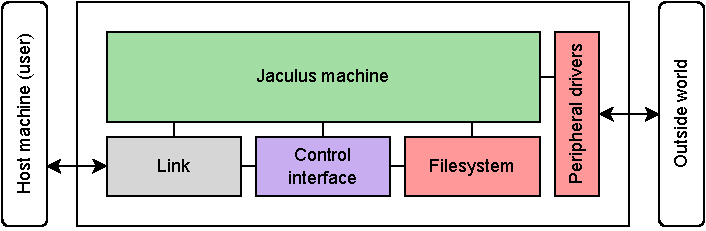
\includegraphics[width=\textwidth]{img/jaculus-design}
  \caption{Structure of the Jaculus firmware}
  \label{fig:jaculus-design}
\end{figure}

The implementation opts for a multithreaded design because continuously interrupting the runtime to poll for new events would slow down the execution of JavaScript code. The JavaScript runtime runs in a separate thread and allows other threads to schedule tasks to be executed in the runtime thread. The main thread then executes these tasks in the order they were scheduled. Separate threads are also used for other tasks, such as communication with the host device. Therefore, most implemented data structures implement blocking operations, allowing these threads to wait for respective events instead of polling for them.


\chapter{Used technologies}

This chapter briefly describes some selected technologies used in the project and some of their specifics.

\section{ESP32 and ESP32-S3}

ESP32\cite{esp32} and ESP32-S3\cite{esp32-s3} are microcontrollers series by Espressif Systems.

ESP32 is a dual-core microcontroller based on the Xtensa LX6 CPU architecture with 520 KiB of SRAM. It features a UART interface for programming.

The ESP32-S3 is a newer iteration of the ESP32 series of microcontrollers. It is based on the Xtensa LX7 CPU architecture and has 512 KiB of SRAM. Aside from a UART interface, it also features a native USB interface, which can be used for programming.

Both of these microcontrollers also provide a Wi-Fi and Bluetooth interface and a large number of other peripherals. On many boards based around these microcontrollers, the programming UART interface is connected to a USB-to-UART bridge, which allows the microcontroller to be programmed over USB. The USB ports are also often used for communication with the program running on the microcontroller.

These microcontrollers are also coupled with flash memory, which stores the firmware and can be used to store other data. The flash memory size varies between individual boards but is usually at least 4 MiB.

\section{ESP-IDF}

ESP-IDF is the official development framework for microcontrollers from Espressif Systems. The framework is based on FreeRTOS and provides a set of libraries and tools for developing applications for, among others, ESP32 and ESP32-S3 microcontrollers.

Most of the libraries provided with ESP-IDF have only a C API. The framework also supports C++20 with a large subset of its standard library. However, some parts of the standard library do not work entirely correctly (e.g., `std::filesystem`).

\section{JavaScript}

JavaScript is a high-level, interpreted, and weakly, dynamically typed programming language. It is standardized in the ECMAScript specification, which is maintained by Ecma International.

Although JavaScript programs are event-driven, the code is executed in a single thread. This is achieved by using an event loop, where asynchronous events are queued and executed in the order they are received. Therefore, JavaScript programs must be written in a non-blocking manner, as blocking the event loop will cause the program to stop responding to events. Events are generated by the JavaScript engine or the host environment both synchronously and asynchronously.

\section{TypeScript}

TypeScript is a strongly typed superset of JavaScript and is developed and maintained by Microsoft. TypeScript is typically not interpreted directly and is instead transpiled into JavaScript, which can be interpreted using any JavaScript runtime that supports the specified ECMAScript version.

\section{QuickJS}

QuickJS is a JavaScript engine implementing the ECMAScript 2020 Language Specification\cite{es2020} (ES2020). It was developed by Fabrice Bellard and Charlie Gordon and is available under the MIT license. It is written in C and is designed to be embeddable into other applications.

QuickJS uses POSIX to implement atomic operations and system time. Although this slightly limits its portability, ESP-IDF, the primary target platform for Jaculus, does support POSIX.

According to ES2020, JavaScript code is evaluated in a *Realm*, which defines the execution environment (e.g., global object and set of built-in objects). QuickJS uses a different term for this concept --- *Context*, which I have adopted for Jaculus and which will be used throughout the rest of this thesis.

Slight modifications have been made to the QuickJS source code to allow it to be compiled with the ESP-IDF toolchain. These modifications do not concern the engine's logic and only change its platform-specific configuration. It has also been extended to work with the CMake and ESP-IDF build systems.


\shorthandon{'}
\end{markdown*}
